\documentclass[titlepage,11pt]{article}

\textwidth 6.5in
\textheight 9in
\oddsidemargin -0.2in
\topmargin -0.5in

\usepackage{indentfirst,graphics,alltt,epsfig,color}

\title{iBioSim Version 2.8 \\ Synthetic Biology Tutorial}

\author{Chris J. Myers}

\begin{document}

\maketitle

%show only subsection granularity in the toc
%\setcounter{tocdepth}{2} 
  
\tableofcontents

\clearpage

\section{Introduction}

\noindent
{\tt iBioSim} has been developed for the modeling, analysis, and design of genetic circuits.  While {\tt iBioSim} primarily targets models of genetic circuits, models representing metabolic networks, cell-signaling pathways, and other biological and chemical systems can also be analyzed.  
{\tt iBioSim} makes extensive use of standard data representations.  Models are specified in {\tt iBioSim} in the %%tth:\begin{html}<A HREF="http://www.sbml.org/">\end{html}
\emph{Systems Biology Markup Language}
%%tth:\begin{html}</A>\end{html}
~(SBML).  It can import all levels and versions of SBML and is able to export Level 3 Version 1.  It supports all core SBML modeling constructs except some types of \emph{fast} reactions, and also has support for the hierarchical model composition, layout, flux balance constraints, and arrays packages.  It was the first tool to produce correct results for all examples in the SBML benchmark suite.  It has also been tested successfully on the stochastic benchmark suite and the curated models in the 
%%tth:\begin{html}<A HREF="http://www.ebi.ac.uk/biomodels-main/">\end{html}
\emph{BioModels database}.
%%tth:\begin{html}</A>\end{html}
{\tt iBioSim} can also import 
%%tth:\begin{html}<A HREF="http://sed-ml.org/">\end{html}
\emph{SED-ML} files 
%%tth:\begin{html}</A>\end{html}
that describe simulation experiments.  Finally, it is one of the first tools to also support the 
%%tth:\begin{html}<A HREF="http://www.sbolstandard.org/">\end{html}
\emph{Synthetic Biology Open Language}
%%tth:\begin{html}</A>\end{html}  
~(SBOL), an emerging standard for information exchange in synthetic biology.

{\tt iBioSim} includes the following components: 

\begin{itemize}
\item Model Editor - a tool to create a model of a genetic circuit or other biological system.
\item SBOL Browser - a tool to view SBOL files and associate DNA components to model elements.
\item Analysis Tool - an abstraction-based ODE, Monte Carlo, and Markov analysis tool.
\item Learn Tool - a tool to learn a model from \emph{time series data} (TSD).
\item TSD Graph Editor- a tool to visualize TSD files. 
\item Histogram Graph Editor - a tool to visualize probability data. 
\end{itemize}

This tutorial illustrates the first three of these features of {\tt iBioSim} using a model of the Genetic Toggle Switch (Gardner et al., 2000).

\section{Project Management}

\noindent
Within {\tt iBioSim}, all files are collected within projects.   A project is a collection of models, analysis views, learn views, and graphs.  As shown below, {\tt iBioSim} displays all project files on the left, the open models, views, and graphs on the right, and a log of all external commands on the bottom.  The menu bar is located on the top of the window in the Windows and Linux versions.  It is located on the top of the screen in the MacOS version.

\begin{center}

\includegraphics[width=160mm]{screenshots/iBioSim}
\end{center}

\noindent
To create a new project, select New $\rightarrow$ Project from the File menu as shown below.  You will then be prompted to browse to a desired location and to give a name to the project directory.  Enter the name {\tt SynBioTutorial}.  After you do this, click the new button and a new project directory will be created.  

\begin{center}
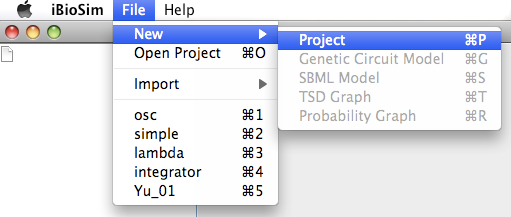
\includegraphics[width=60mm]{screenshots/project}
\end{center}

\section{Importing Models}

\noindent
In order to do analysis within {\tt iBioSim}, you must first have models to analyze.  The simplest way to obtain a model to analyze is to import it from an external source.  As shown below, using the menu option File $\rightarrow$ Import, {\tt iBioSim} can import models in a variety of ways.  First, one can simply import an SBML model from somewhere on the local file system.  

\begin{center}
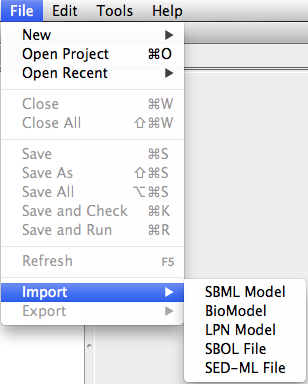
\includegraphics[width=60mm]{screenshots/import}
\end{center}

One can also import an SBML model from the EMBL-EBI's BioModels Repository by selecting the menu option File $\rightarrow$ Import $\rightarrow$ BioModel.  This brings up the window shown below without the model names.  Pressing the Get Names button will fetch the names, but this takes awhile the first time, so let's skip that for now.  Instead, scroll down to BIOMD0000000507 and Press the Get Description button which brings up the BioModels entry for this model in a browser, which you can see is the original model of the genetic toggle switch.  The Get Reference button brings up a browser entry for the original publication.  With BIOMD0000000507 highlighted, press OK to fetch this SBML model.  Since this model does not include any layout information, you will need to either lay it out by hand or use one of the default layout routines selectable using the Apply Layout icon 
\includegraphics{../gui/icons/modelview/choose_layout_selected}.  Horizontal Hierarchical layout works well for this model.  Click on the ``X'' to close the window.

\begin{center}
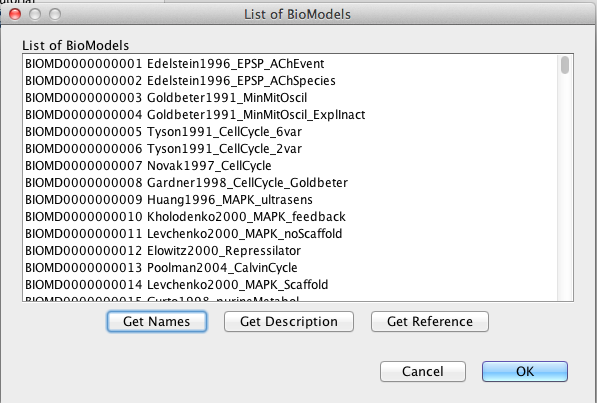
\includegraphics[width=120mm]{screenshots/BioModels}
\end{center}

Another source for import of SBML models is from Newcastle University's Virtual Parts Repository.  In this case, you can either import a model of the part or of the part's interactions.  

\begin{center}
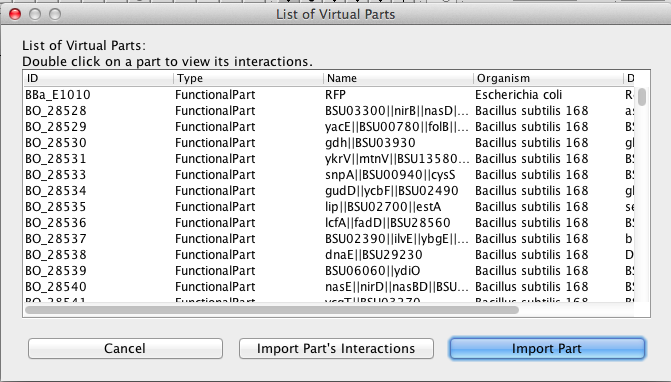
\includegraphics[width=120mm]{screenshots/VirtualParts}
\end{center}

Next, you can import a \emph{labeled Petri net} (LPN) model.  Petri net models are a type of discrete modeling formalism similar to a state machine though with more support for the modeling of concurrent systems.  LPNs extend Petri nets with labels that indicate when state transitions are enabled, the time they take, and how they update the system state.  {\tt iBioSim} uses the LPN format for Markov chain analysis of biological systems.  

We can also import an SBOL file that provides annotated DNA sequences for DNA components.  More on this later.  

Finally, we can import a SED-ML file that describes a simulation experiment. 
Importing a SED-ML file will also import the SBML models required for the simulation followed by performing the simulation.   To see how this works, select File $\rightarrow$ Import $\rightarrow$ SED-ML File, and browse to the install directory for {\tt iBioSim}.  Continue browsing from here to the directory:\\
{\tt <INSTALL DIRECTORY>/docs/SynBioTutorial/SBMLTestSuite} \\
which contains the SBML testsuite files.  Go to test 00001, and select the file:\\
{\tt 00001-sbml-l3v1-sedml.xml}.  This will import an SBML model called {\tt case00001.xml} and simulate it.  Click on the tab labelled TSD Graph to see the result of an ODE simulation of this model.  Repeat these steps to import a SED-ML file for test case 01195.  This SBML model is a \emph{flux balance} model, so the analysis performed is flux balance analysis.  To see the results, click on the Histogram tab.  Now, click on the ``X'' to close each window.

\begin{center}
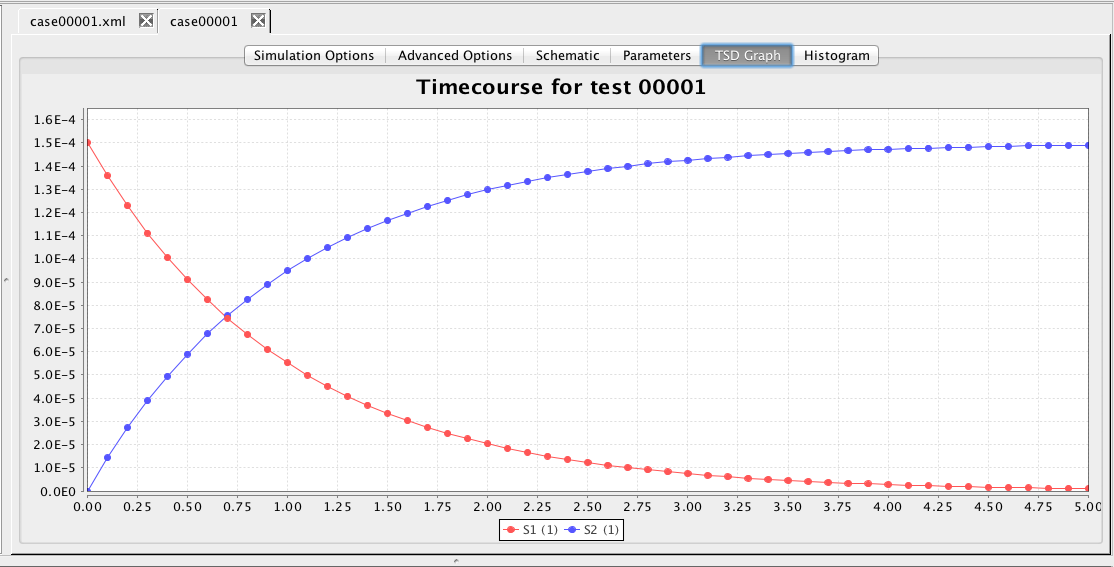
\includegraphics[width=160mm]{screenshots/TestSuiteResults}
\end{center}

\begin{center}
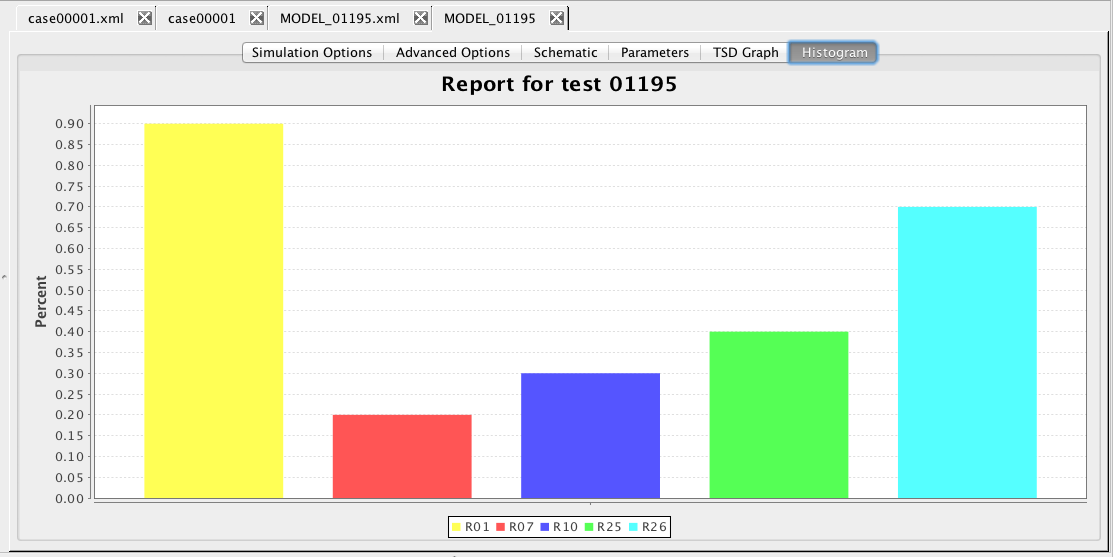
\includegraphics[width=160mm]{screenshots/FBAresults}
\end{center}

\section{Model Editor}

\noindent
Let us know see how to create a new model using the Model Editor.  First, select New $\rightarrow$ Model from the File menu as shown below. You will then be prompted to enter a model ID.  Enter {\tt LacI\_Inverter}.  At this point, a Model editor will open in a new tab.

\begin{center}
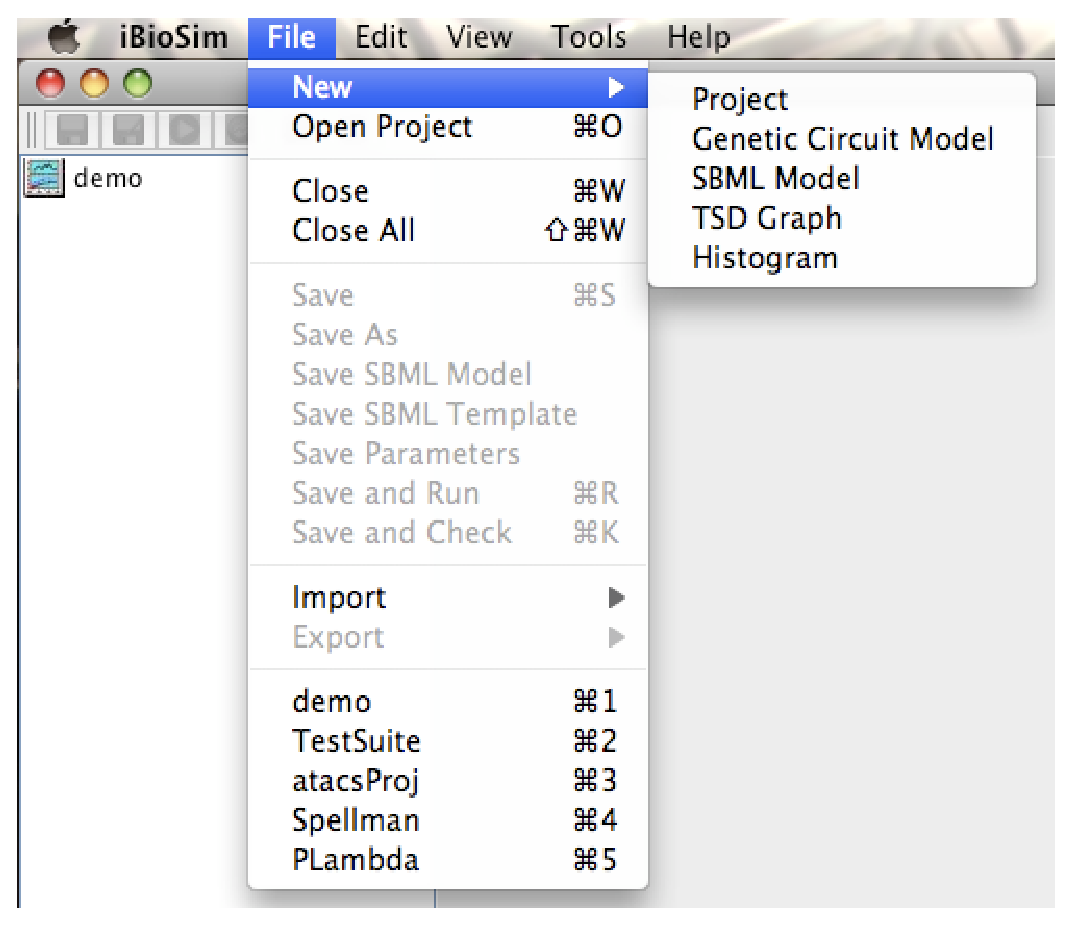
\includegraphics[width=80mm]{screenshots/newModel}
\end{center}

\begin{center}
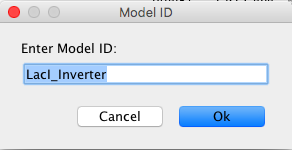
\includegraphics[height=25mm]{screenshots/ModelIdGT}
\end{center}

\begin{center}
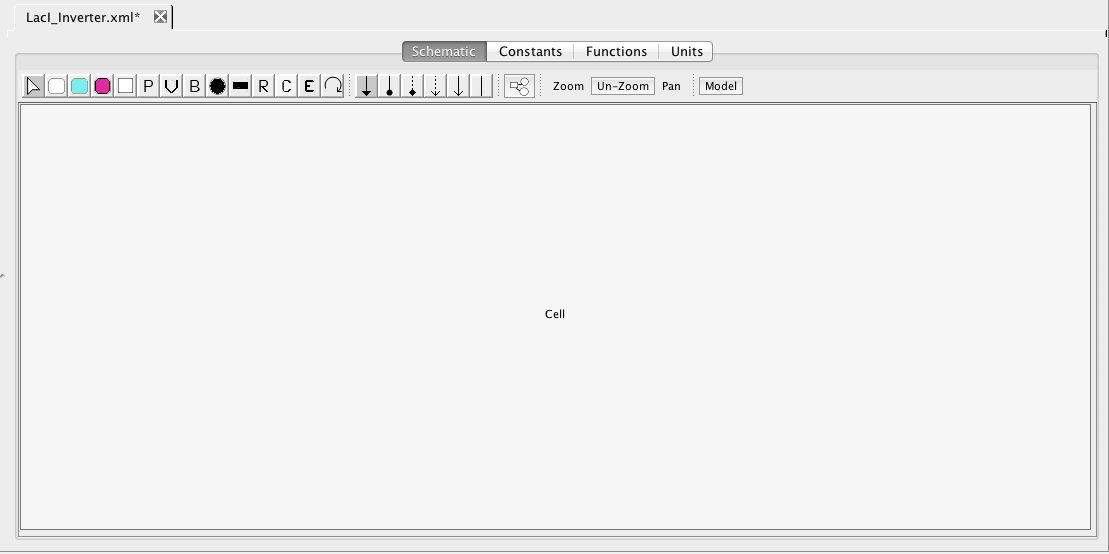
\includegraphics[width=160mm]{screenshots/schematicGT}
\end{center}

To add a chemical species, select the Add Species icon 
\includegraphics{../gui/icons/modelview/add_species_selected} and click on the schematic canvas  (note that this can also be done using the Edit menu or the hotkeys shown in this menu).  This will drop a new species with default ID and other values.  You may change these defaults by clicking on the selection icon 

\includegraphics{../gui/icons/modelview/select_mode_selected}, and
double-clicking on the species to open the Species Editor.  In this case, let us change the ID to LacI and change the Port type to \emph{input}.  We will leave all the other values at their default values.  The port type of input indicates that this species will be used as an input for the LacI inverter.   
Note that while in the select mode, you can also select an object in the schematic and move it by moving the mouse while holding the left mouse button.  Pressing the right mouse button while an object is selected brings up a menu that allows you to delete an object from the schematic.  Repeat the steps above to add TetR and GFP species.  Give these species port type of \emph{output}. 

\begin{center}
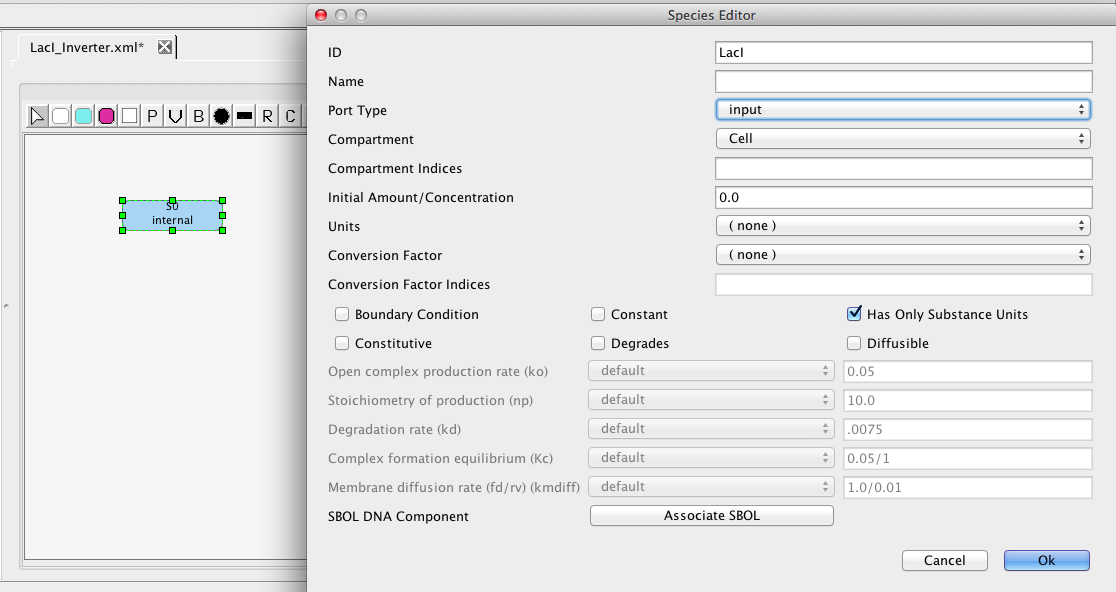
\includegraphics[width=160mm]{screenshots/speciesGT}
\end{center}

% Add another species for the CI dimer molecule.  The next step is to add a complex-formation reaction to convert CI monomers into CI dimers.  Select the complex formation icon 
\includegraphics{../gui/icons/modelview/bio_activation_selected}, highlight the CI species, and, while holding the mouse button, stretch the complex formation arc to the S1 species.  Next, edit this species to set its ID to CI2 and select that it degrades.  This species is created using a complex-formation reaction with an equilibrium constant of 0.1.  Change default to custom for the complex formation equilibrium and set it to this value as shown below.

% \begin{center}
% 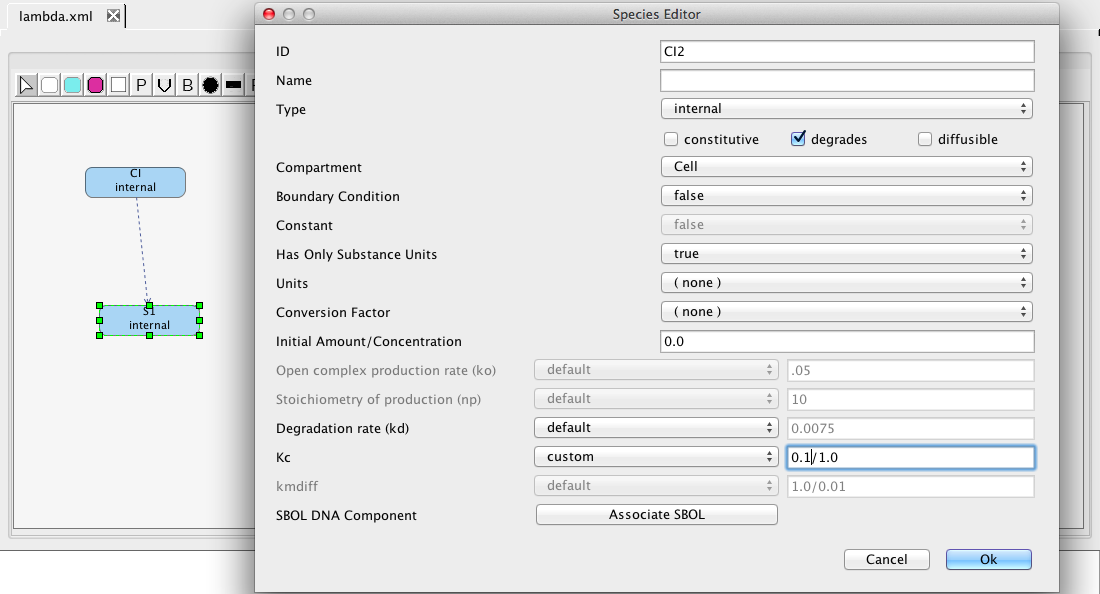
\includegraphics[width=160mm]{screenshots/species2} 
% \end{center}

% If you double-click on the complex formation arc, an influence editor will open which indicates that this is a complex formation arc and the stoichiometry of binding (i.e., the number of molecules of the source species used to construct the sink species) is 2.  The default in this case is correct as it does take two molecules of CI to make CI2.

% \begin{center}
% 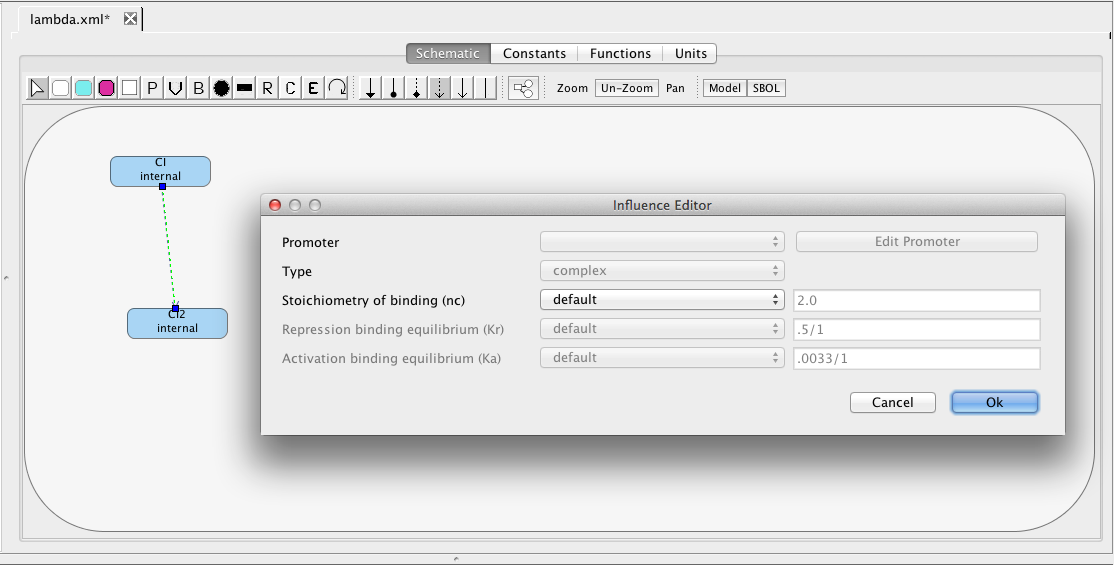
\includegraphics[width=160mm]{screenshots/complex} 
% \end{center}

Next, let's add the pLac promoter, which initiates transcription of the gene that produces the proteins TetR and GFP.  To do this, select the promoter icon 
\includegraphics{../gui/icons/modelview/promoter_mode_selected} and click on the schematic canvas to drop the promoter with a default ID and parameter values.  Double-click on the promoter to bring up the promoter editor.  Change the ID to pLac.
 
\begin{center}
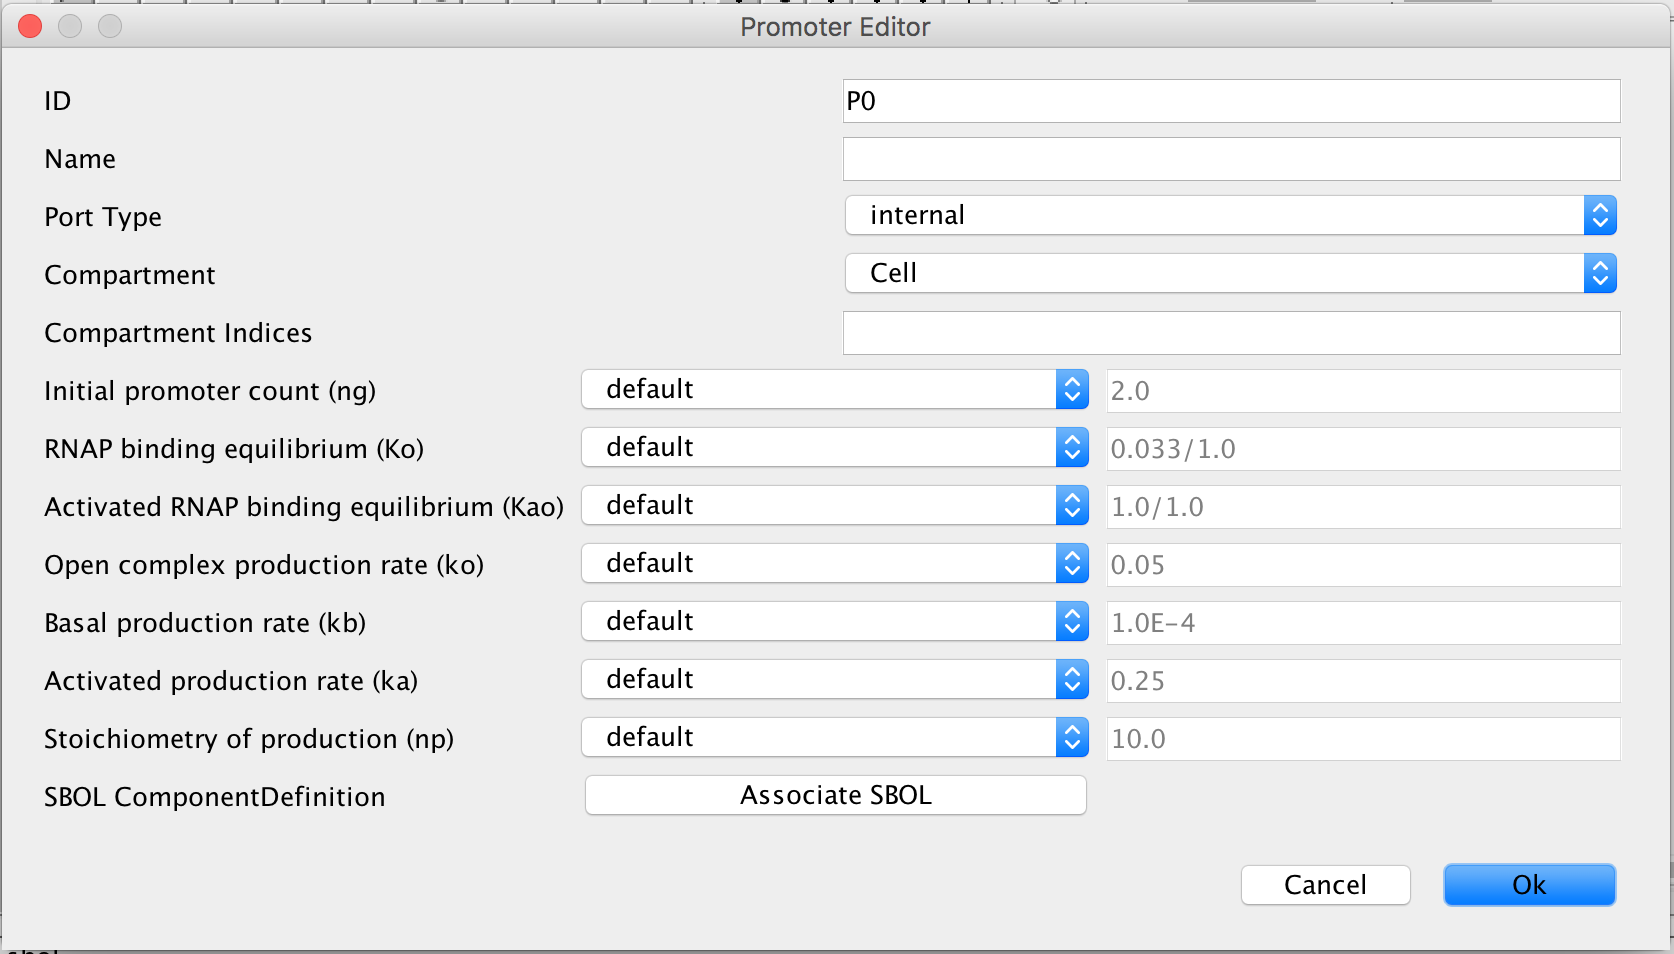
\includegraphics[width=160mm]{screenshots/promoterGT} 
\end{center}

The pLac promoter is repressed by the LacI species.  To create this relationship, select the repression arc icon 

\includegraphics{../gui/icons/modelview/inhibition_selected}, highlight the LacI species, and, while holding the mouse button, stretch the repression arc to the pLac promoter.  
%% Next, double-click on the repression arc to bring up the influence editor.  

\begin{center}
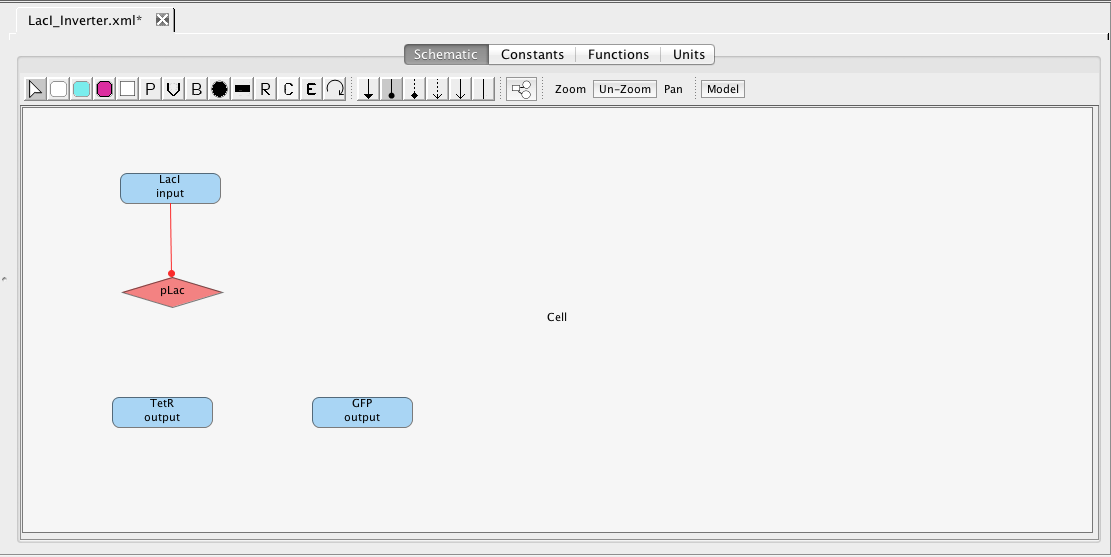
\includegraphics[width=160mm]{screenshots/repressionGT} 
\end{center}

As mentioned earlier, the pLac promoter initiates the production of the TetR and GFP species.  Highlight the pLac promoter and, while holding the mouse button, stretch the production arc to the TetR species.  Repeat these steps to create a production arc between the pLac promoter and GFP species.  Note that any regulation icon can be selected for this because all arcs from promoters to species are always production arcs.  

\begin{center}
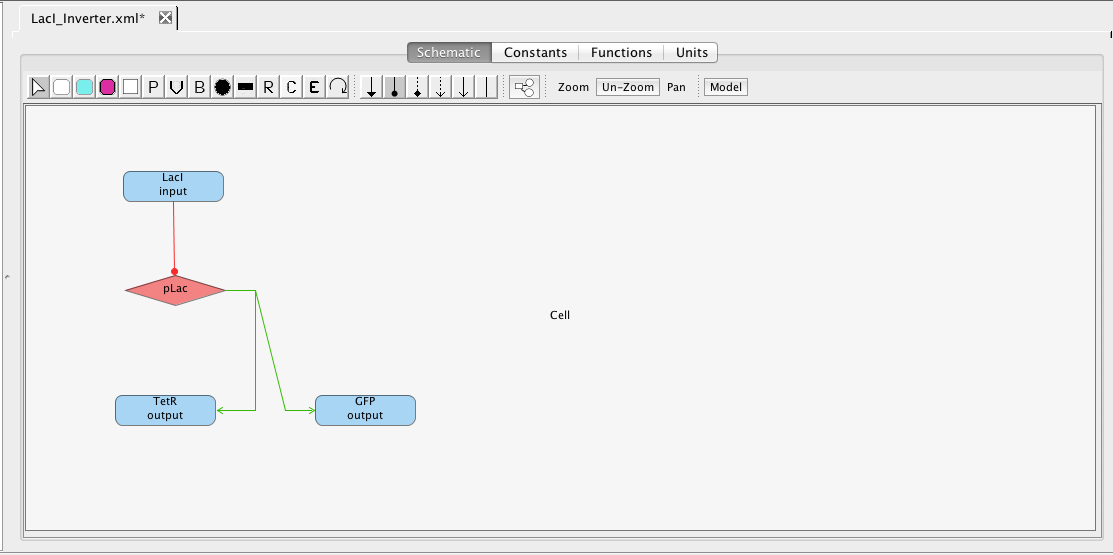
\includegraphics[width=160mm]{screenshots/productionGT}
\end{center}

Let us now annotate the LacI inverter with its DNA sequence.  To do this, we will need to first import some annotated sequence data stored using the \emph{synthetic biology open language} (SBOL).  Select the File $\rightarrow$ Import $\rightarrow$ SBOL File menu option as shown below.  This will bring up a file browser.  You will need to find the location where {\tt iBioSim} is installed, and the file you want to import should be located in {\tt iBioSim/docs/SynBioTutorial/SBOL/GeneticToggle.sbol}.  

\begin{center}
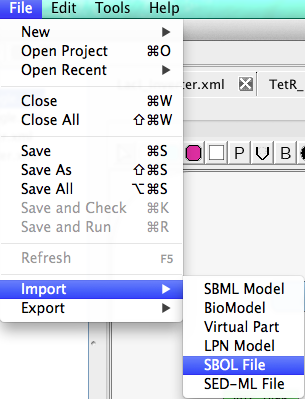
\includegraphics[width=60mm]{screenshots/importSBOL}
\end{center}

Next, click on the Model button in the schematic editor which brings up the Model editor shown below.  

\begin{center}
\includegraphics[width=160mm]{screenshots/ModelEditorGT}
\end{center}

Next, click on the Associate SBOL button, highlight the placeholder for the DNA component, and click the Remove button.  Then, press the Add button which will open the SBOL browser shown below.  In the list of DNA components, scroll down to the component named pIKERightCassette\_1, select it, and press OK.

\begin{center}
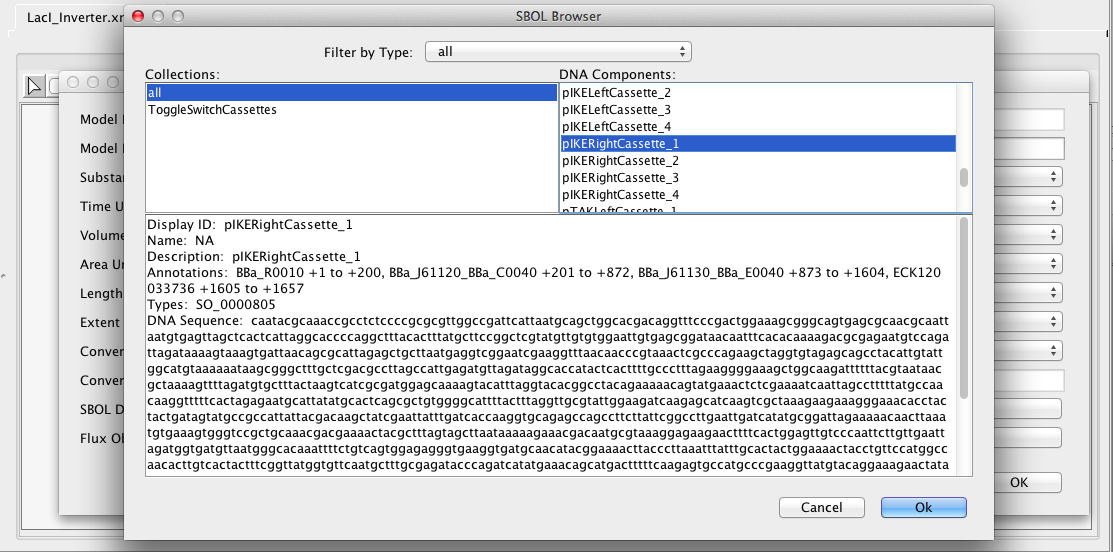
\includegraphics[width=160mm]{screenshots/SBOLBrowserGT}
\end{center}

The SBOL association editor should now show this DNA component as being associated with this model.  We could now add more components, if we wish, but only one is needed for this, so press Ok.  We are now done with the LacI inverter model, so let's make sure the model is saved by either clicking on the Save icon 
\includegraphics{../gui/icons/save} or selecting the Save option from the File menu.

\begin{center}
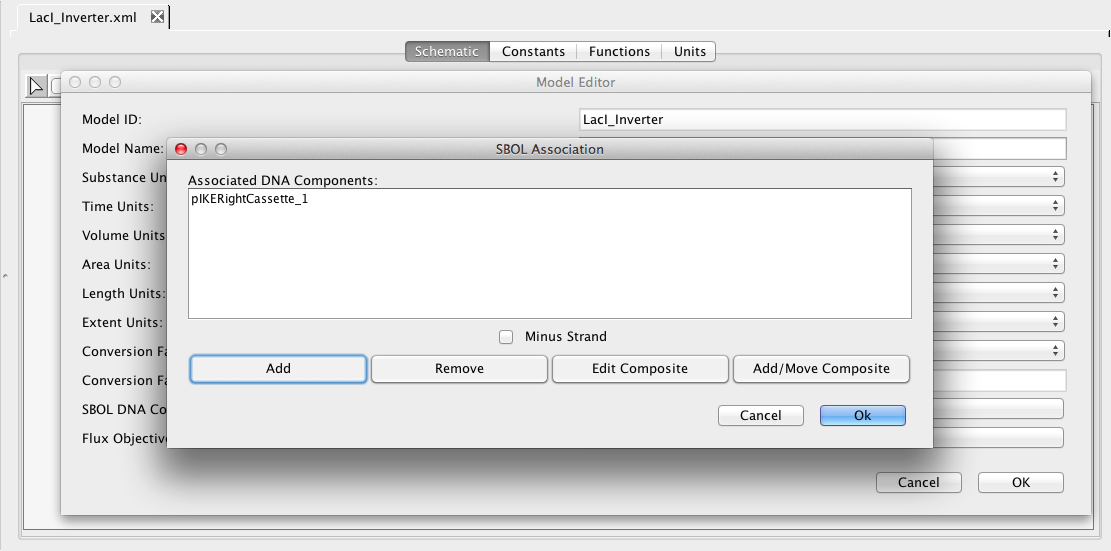
\includegraphics[width=160mm]{screenshots/SBOLAssociationGT}
\end{center}

Next, repeat the steps above to create a TetR\_Inverter model.  The TetR inverter has input TetR and output LacI.  In the TetR inverter, TetR represses the production of LacI.  To indicate this, select the repression icon 
\includegraphics{../gui/icons/modelview/inhibition_selected}, highlight the TetR species and stretch the arc to the LacI species.  This action creates an implicit promoter P0 that is repressed by TetR and initiates production of LacI.  When you associate SBOL with this model, select the pIKELeftCassette\_1 component, and select for it to be put on the Minus Strand by checking the box on the SBOL association window.  Do not forget to save this model either by clicking on the Save icon 
\includegraphics{../gui/icons/save} or selecting the Save option from the File menu.

\begin{center}
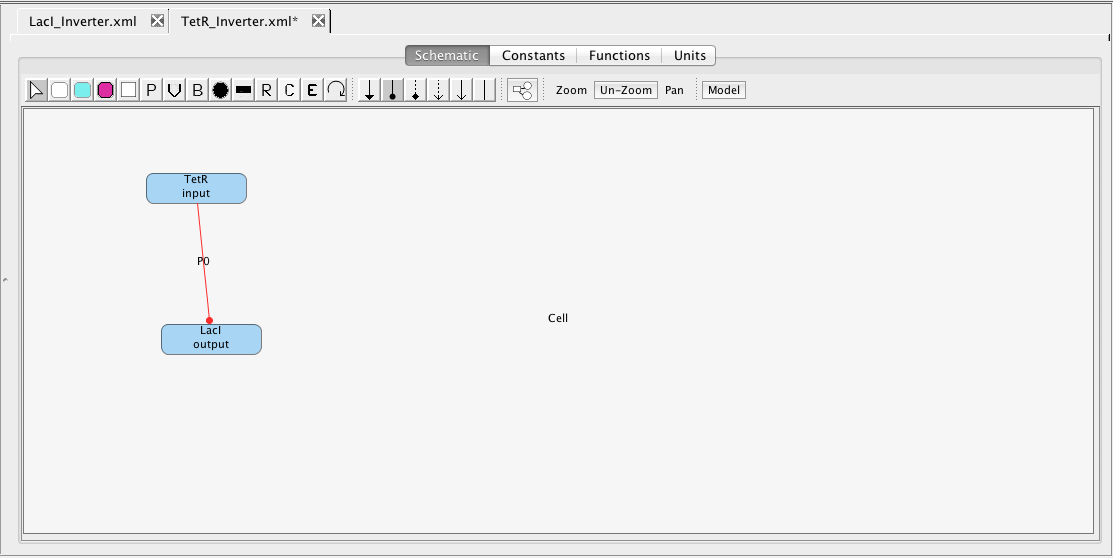
\includegraphics[width=160mm]{screenshots/implicitPromoterGT}
\end{center}

Now, let us put these genetic inverters into a new model called GeneticToggle.
This model will be the top-level model, and all elements of this model will be enclosed in this model's \emph{compartment}.  Compartments are the membrane-enclosed regions where species can be found and reactions take place.  {\tt iBioSim} creates a default compartment initially with the ID of Cell.  If you click on the schematic within the Cell compartment, it brings up the compartment editor.  Uncheck the ``Is Mapped to a Port''.  This indicates that this compartment should be enclosing this model and not replaced when instantiated in a larger model.  Once you press OK, you will notice that the compartment now has rounded corners to indicate that this is membrane enclosed by the compartment Cell.

\begin{center}
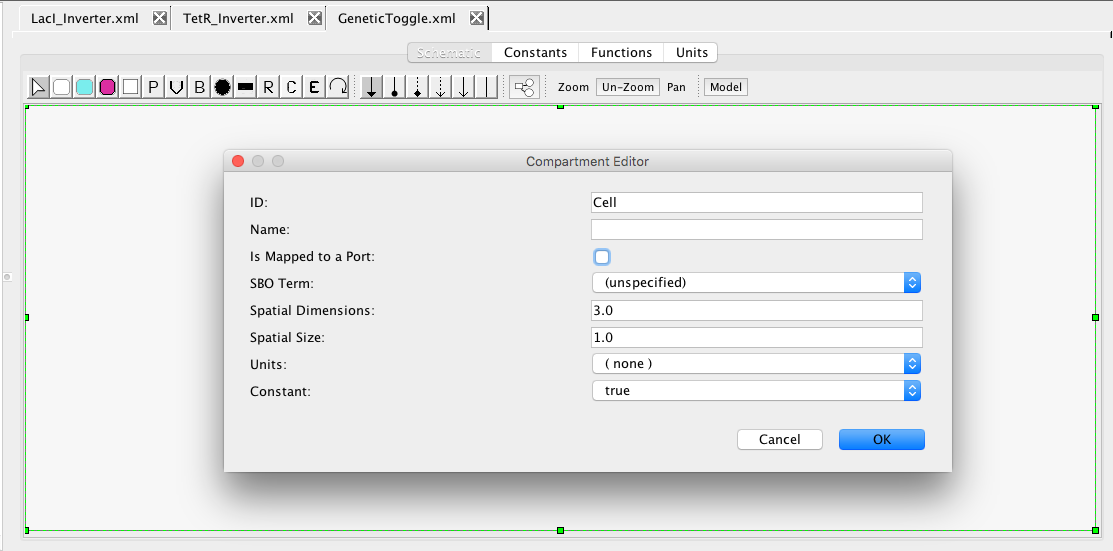
\includegraphics[width=160mm]{screenshots/compartmentGT}
\end{center}

Now, lets add the LacI\_Inverter component to this model.  Select the Add Component icon 
\includegraphics{../gui/icons/modelview/add_component_selected} and click on the Schematic canvas opening the Add Component(s) window.  In this window, browse the combo box, if necessary, to find your LacI\_Inverter model.  Pressing OK will then add it to your schematic.  Repeat these steps to add the TetR\_Inverter.

\begin{center}
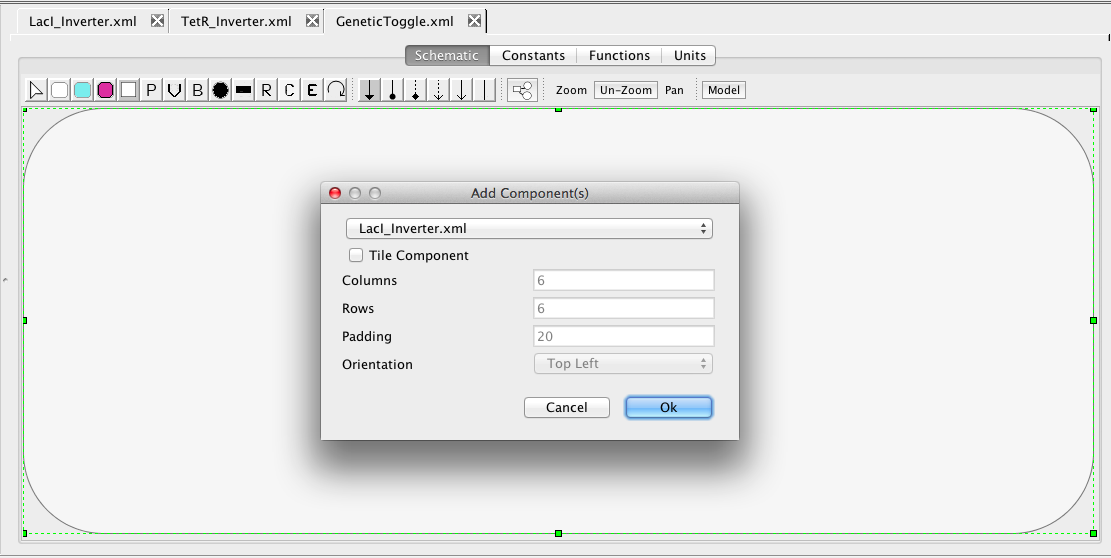
\includegraphics[width=160mm]{screenshots/subModelGT}
\end{center}

The next step is to connect the components through their species.   To do this, add species to the model for LacI, TetR, and GFP.  Mark that each of these species degrades, and set the initial amount of LacI to 60.  The degrades checkbox means that when this model is analyzed a default degradation reaction will be created which has a rate of 0.0075.  Next, highlight the LacI species and stretch a connection to the LacI\_Inverter connecting it to its LacI input port.  Next, highlight the LacI\_Inverter and stretch to the TetR species.  In this case, since there are two output ports, you must select the TetR output port is the one desired.  Next, highlight the TetR species and stretch to the TetR\_Inverter to connect to the TetR input port.  Next, highlight the TetR\_Inverter and stretch to the LacI species to connect it to its LacI output port.  Finally, highlight the Lac\_Inverter and stretch to the GFP species being sure to select to connect to its GFP output port.  

\begin{center}
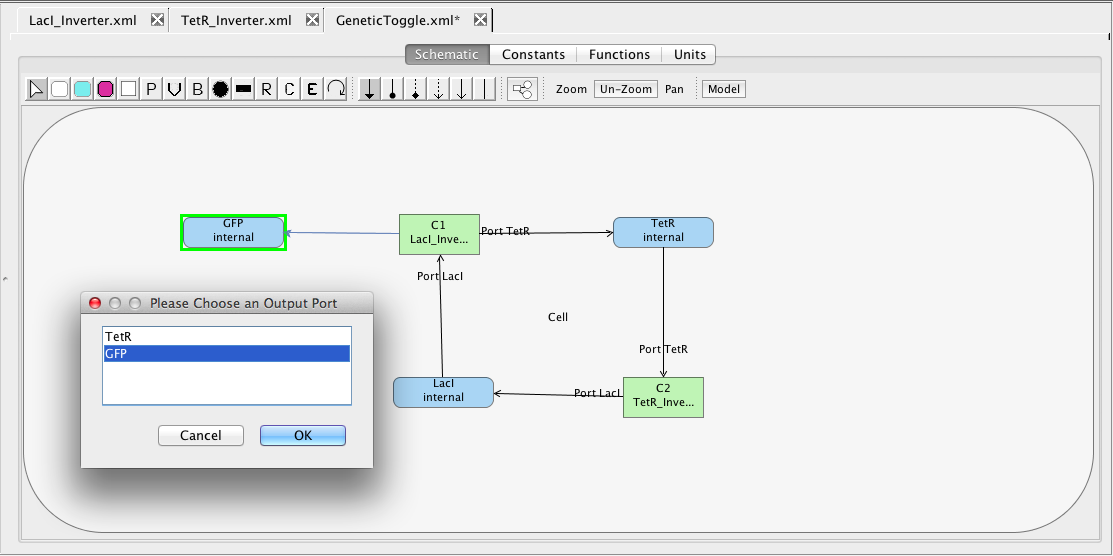
\includegraphics[width=160mm]{screenshots/addConnectionGT}
\end{center}

By instantiating these models together, the SBOL associated with each component will now be composed as well.  To add some description for this composite DNA component, click on the Model button, followed by the Associate SBOL button on the Model Editor, and finally the Edit Composite button on the SBOL Association window.  You can now add an ID, Name, and Description for this composite DNA component as shown below.  

\begin{center}
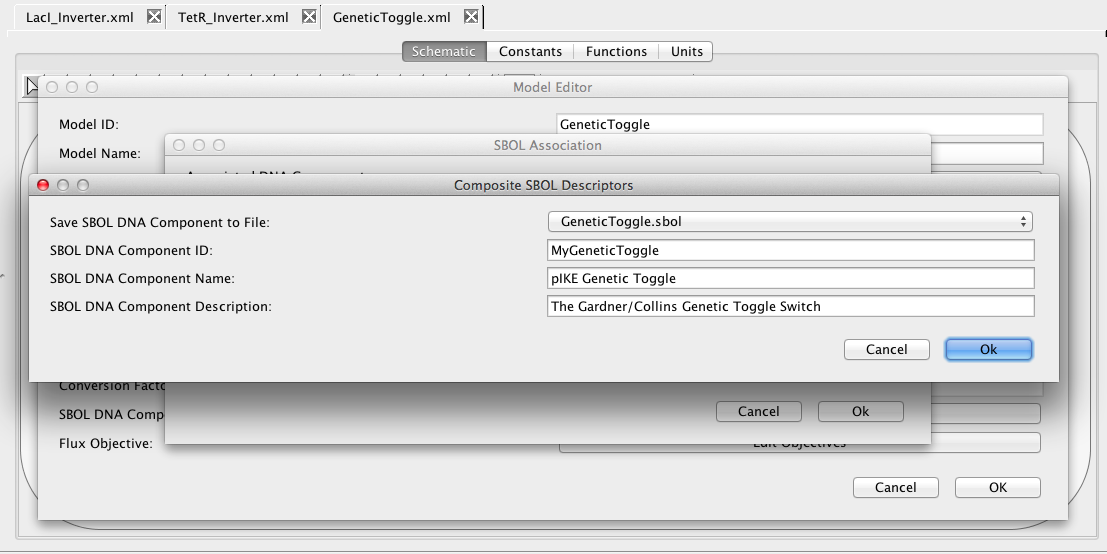
\includegraphics[width=160mm]{screenshots/compSBOLDesc}
\end{center}

Next let us add the complex formation reactions that sequester LacI and TetR preventing them from acting as repressors.  First, add the small molecule species IPTG and aTc.  Select \emph{boundary condition} to indicate they are replenished inputs to the system.  Next, add the complex species IPTG\_LacI and aTc\_TetR and mark that they degrade.  Now, select the complex formation icon 
\includegraphics{../gui/icons/modelview/bio_activation_selected}, highlight the IPTG species, and, while holding the mouse button, stretch the complex formation arc to the IPTG\_LacI species.  Repeat this step to connect complex formation arcs between LacI and this complex, as well as from aTc and TetR to the aTc\_TetR complex.  Finally, click on the selection icon 

\includegraphics{../gui/icons/modelview/select_mode_selected}, and
double-click on each complex formation to open the Influence Editor.  In this editor, change the Stoichiometry of binding (nc) from 2 to 1 by first changing ``default'' to ``custom'' then editing the value.

\begin{center}
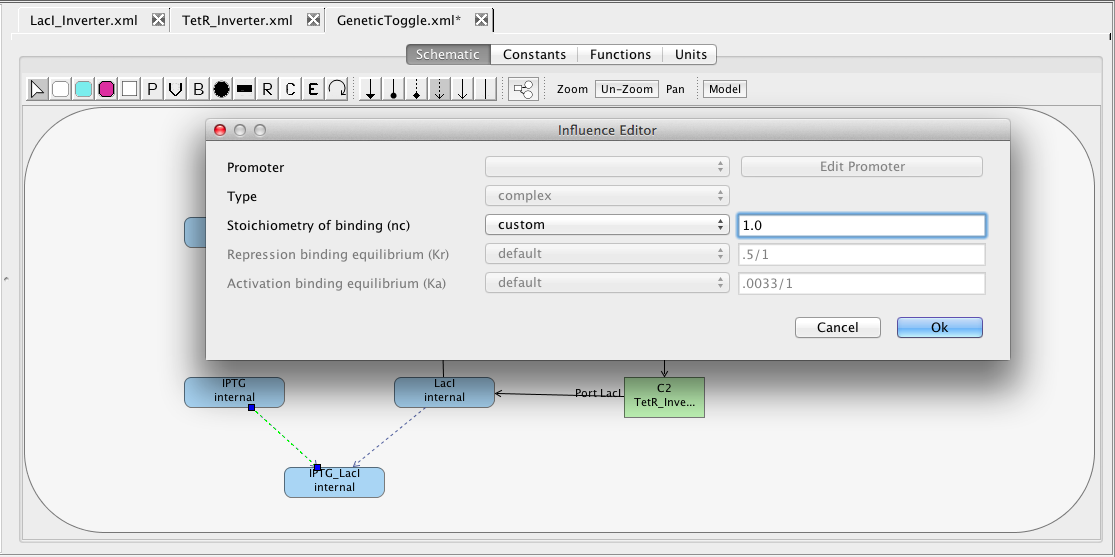
\includegraphics[width=160mm]{screenshots/complexGT}
\end{center}

The final step in the model creation is to add some discrete events to change the amounts of IPTG and aTc, so we may see the genetic toggle switch change state during simulation.  First, select the event icon 
\includegraphics{../gui/icons/modelview/event_mode_selected}, and click on the schematic to add an event.  This action opens the event editor.  In this editor, create an event with ID ``IPTG\_High'', a trigger of ``true'', and a delay of 2000.  Next, click on Add Assignment to bring up the Event Assignment Editor.  In this editor, select the variable IPTG and provide the assignment of 60.  Press the Add button to add the assignment and the Add button to add the event.  This event will cause the amount of IPTG to change to 60 molecules after 2000 seconds of simulation time.  Repeat these steps to create an ``IPTG\_Low'' event with a delay of 4000 which assigns 0 to IPTG, an ``aTc\_High'' event with a delay of 6000 which assigns 60 to aTc, and finally an ``aTc\_Low'' event with a delay of 8000 which assigns 0 to aTc.

\begin{center}
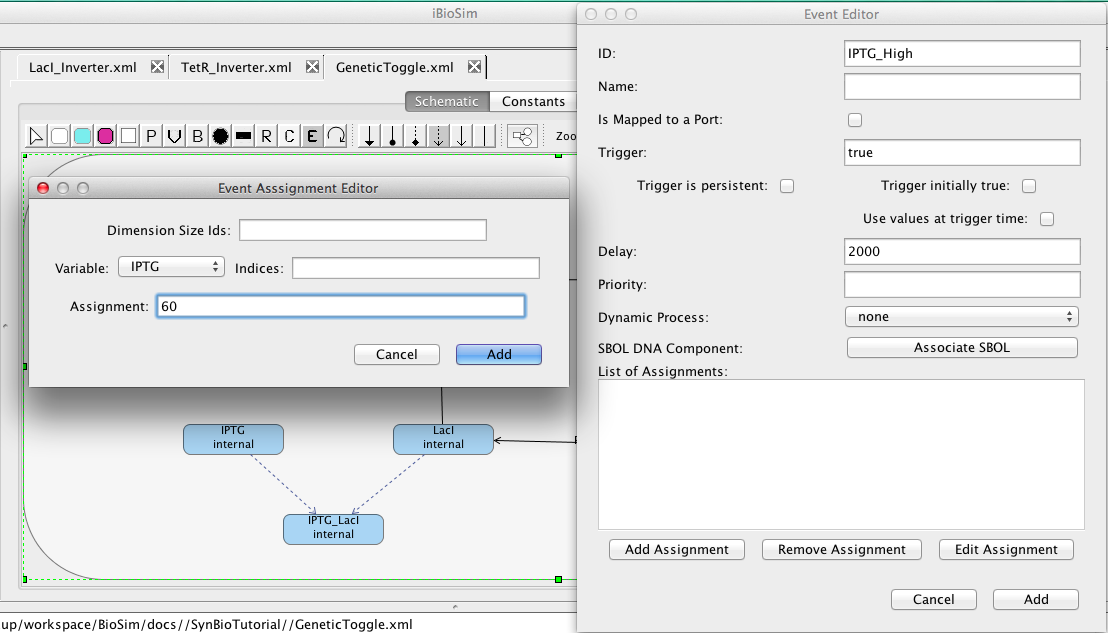
\includegraphics[width=160mm]{screenshots/eventGT}
\end{center}

You should now have a complete model of the genetic toggle switch that looks like the one below (though locations of elements may be different).  Make sure the model is saved by either clicking on the Save icon 
\includegraphics{../gui/icons/save} or selecting the Save option from the File menu.

\begin{center}
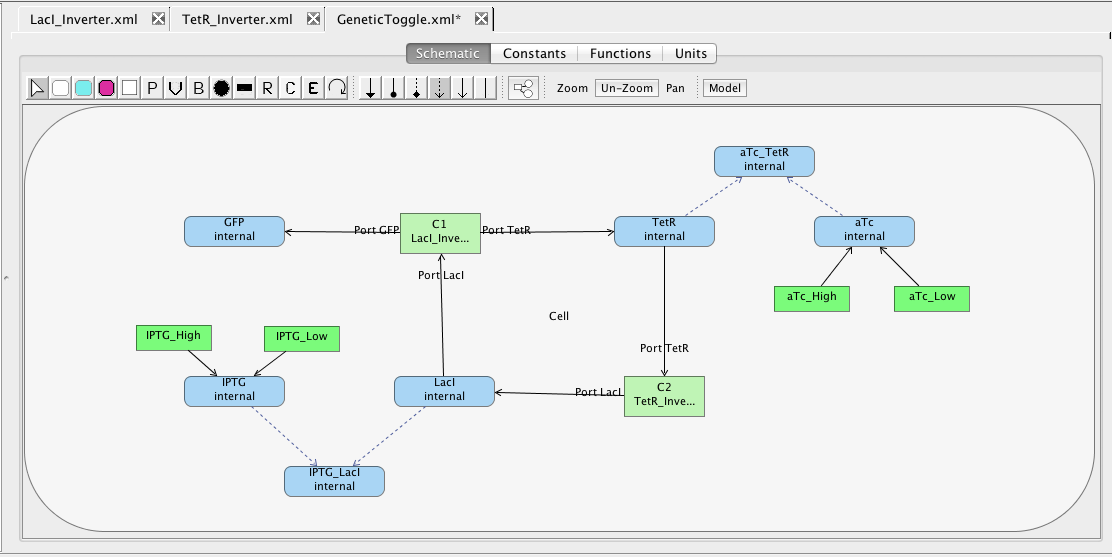
\includegraphics[width=160mm]{screenshots/saveGT}
\end{center}

\section{SBOL Browser}

As mentioned above, a composite DNA component has been constructed for the entire genetic toggle switch.  To see this component, click on the GeneticToggle.sbol file in the list of project files to open the SBOL browser.  On the right side, scroll down and select the DNA component that you named MyGeneticToggle.  You will now see the complete annotated DNA sequence for this component.  Note how the pIKELeftCassette\_1 has been put on the minus strand while the pIKERightCassette\_1 follows it on the positive strand.

\begin{center}
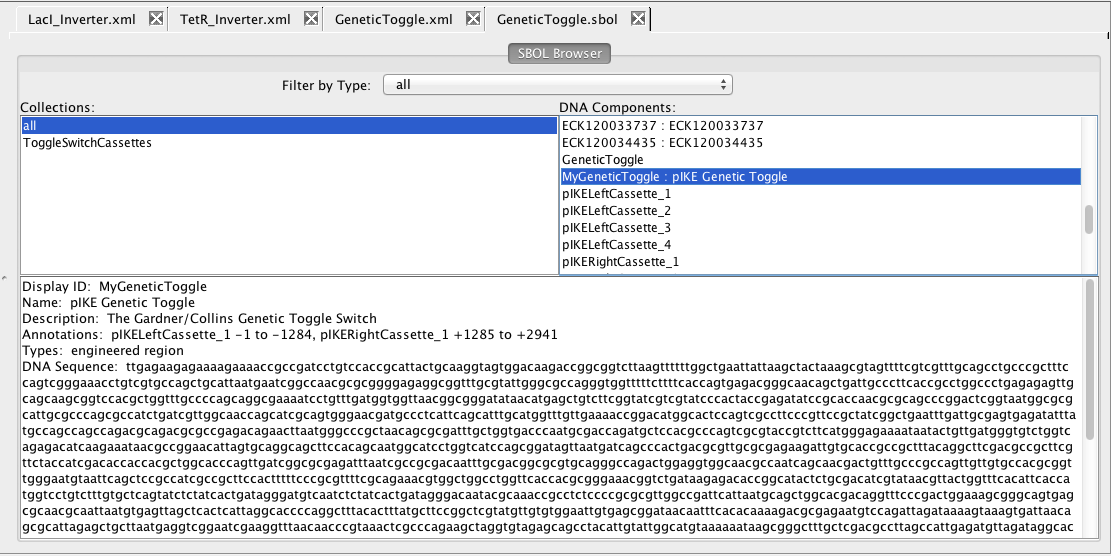
\includegraphics[width=160mm]{screenshots/SBOLBrowserGT2}
\end{center}

\section{Analysis Tool}

This section describes how to analyze the model just created.  The first step is to create an analysis view.  To do this, right-click on the model file and select Create Analysis View.  Enter the analysis ID {\tt GeneticToggle} or just press enter.  At this point, a new analysis view should open.  You should also notice that an icon appears next to your model file.  When you click on this, it will show you all of the analysis and learn views associated with this model.

\begin{center}
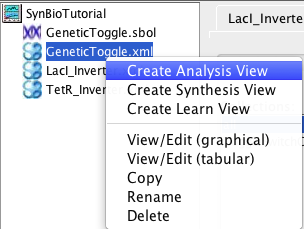
\includegraphics[height=60mm]{screenshots/createAnalysisViewGT}\\
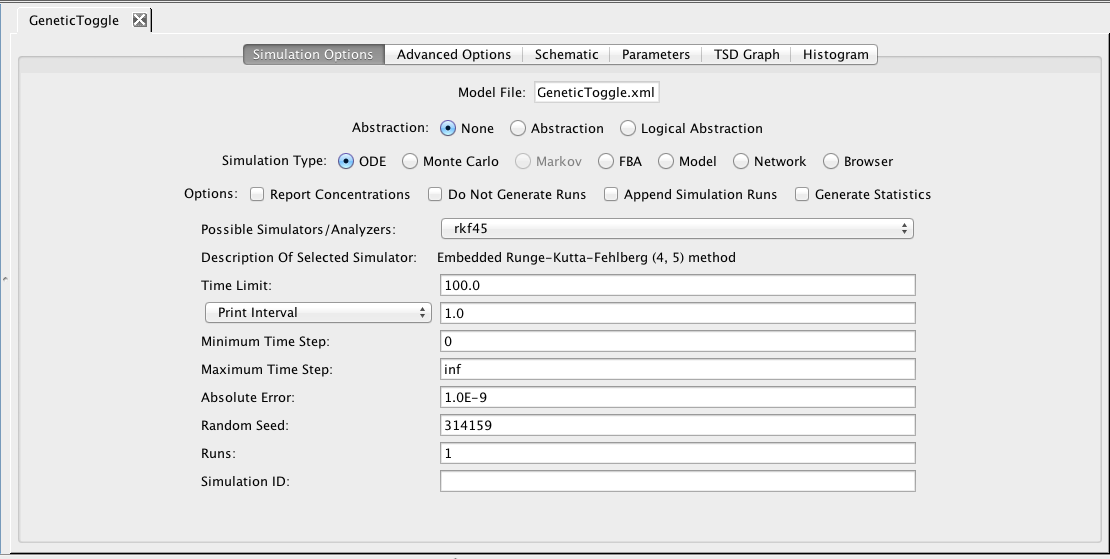
\includegraphics[width=160mm]{screenshots/analysisViewGT}
\end{center}

In order to perform analysis, the analysis tool first converts the model into a detailed reaction-based model.  There are three different ways to see the reaction-based model that is produced.  If GraphViz is installed on your computer, you can select Network for your Simulation Type.  Then, either press the Save and Run icon 
\includegraphics{../gui/icons/run-icon} or select the Save and Run option from the File menu.  The result will be a GraphViz window that will open to show the reaction-based model such as the one shown below for our example.  If it does not open in GraphViz, make sure that you have files with the {\tt .dot} file extension associated with GraphViz on your computer.  You can also view the model in a web browser by selecting Browser for your simulation type.  In this case, you should ensure that you have files with the {\tt .xhtml} extension associated with your favorite browser.  Finally, you can save the reaction-based model by selecting Model as your simulation type.  In this case, you must provide a new model ID.  This new model will appear in your project and it can be opened in the Model Editor.  Since this model does not include any layout information, you will need to either lay it out by hand or using one of the default layout routines selectable using the Apply Layout icon    
\includegraphics{../gui/icons/modelview/choose_layout_selected}.

\begin{center}
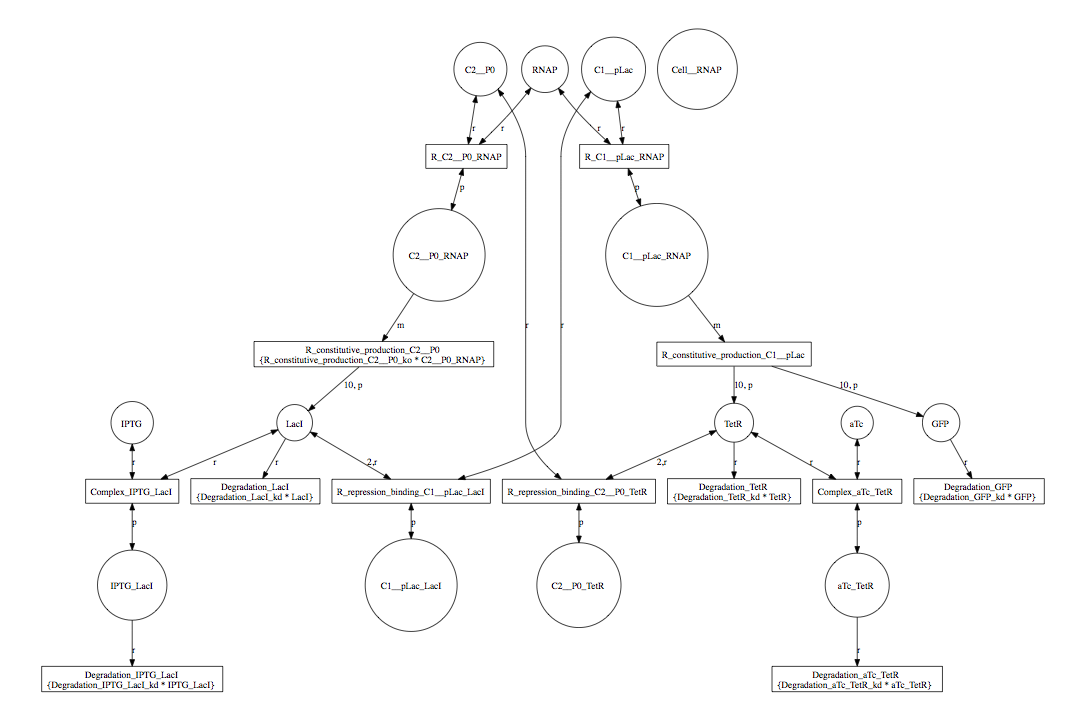
\includegraphics[width=160mm]{screenshots/viewNetworkGT}
\end{center}

\begin{center}
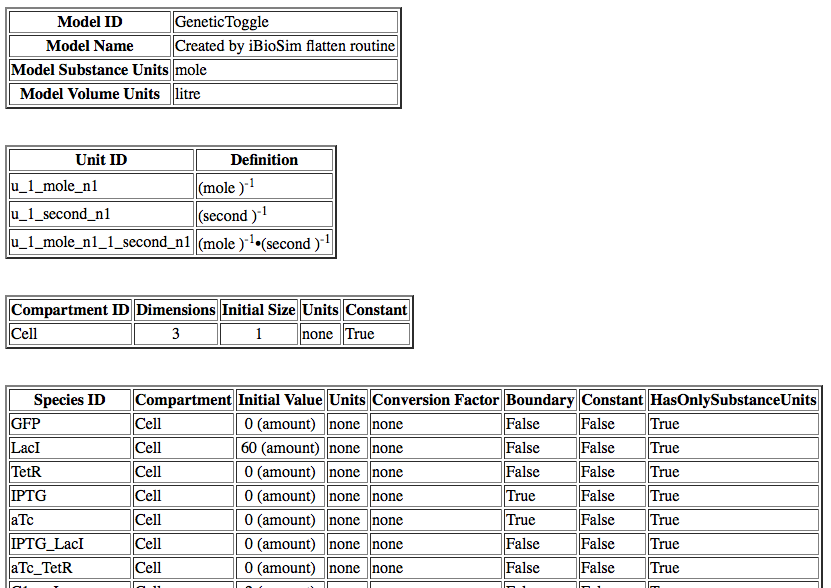
\includegraphics[width=160mm]{screenshots/viewBrowserGT}
\end{center}

\begin{center}
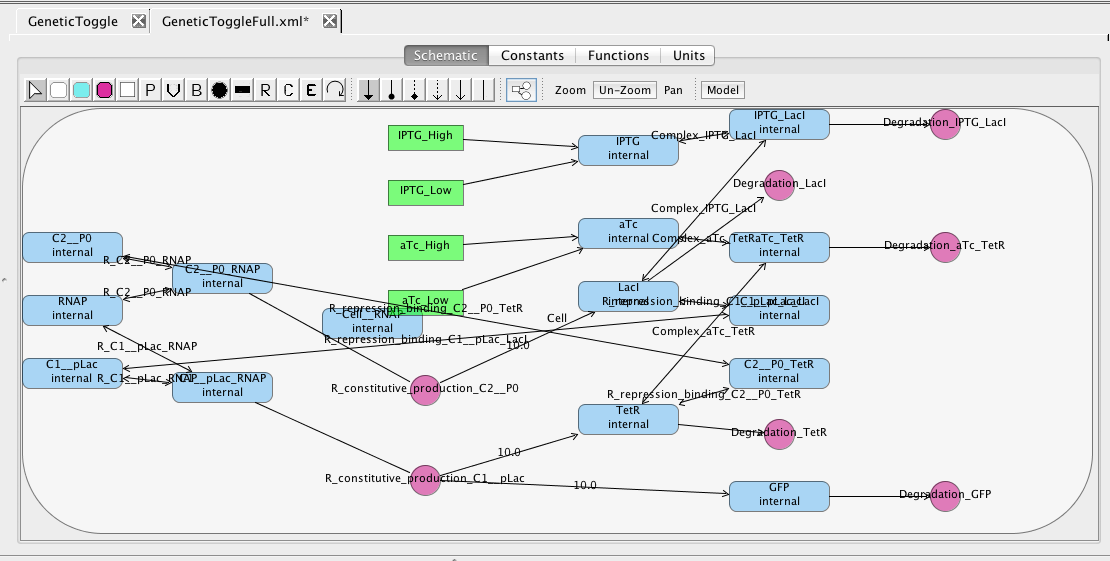
\includegraphics[width=160mm]{screenshots/reactionModelGT}
\end{center}

As you can see, this model is quite complex.  A simple model can be generated by selecting Abstraction to reduce the model using reaction-based abstractions based on the quasi-steady state assumption.  The abstracted model shown below is reduced from 15 species and 13 reactions to just 5 species and 5 reactions.  

\begin{center}
\includegraphics[width=160mm]{screenshots/reactionModelAbsGT}
\end{center}

Now, go back to the simulation options tab.  Here, make sure that Abstraction is still selected, change the simulation type back to ODE, the simulator to Runge-Kutta-Fehlberg,  the time limit to 10000.0, the print interval to 100.0, and enter a Simulation ID of {\tt ode}.  Then, either press the Save and Run icon \includegraphics{../gui/icons/run-icon} or select the Save and Run option from the File menu.
After the simulation completes, click on the TSD Graph tab.  Double-click on the graph to bring up the graph editor.
Open the {\tt ode} simulation, highlight Average, select aTc, IPTG, and GFP, change the Title to ``ODE Simulation Results'', change the X-Axis Label to ``Time (seconds)'', and change the Y-Axis Label to ``Number of Molecules''.  
Press the OK button.  

\begin{center}
\includegraphics[width=160mm]{screenshots/odeSimGT}\\
\includegraphics[width=160mm]{screenshots/odeResultsGT}\\
\includegraphics[width=160mm]{screenshots/odeSimResultsGT}
\end{center}

Graphs can be exported in a variety of formats including:
\begin{itemize}
\item Time series data format (tsd).
\item Comma separated value (csv).
\item Column separated data (dat).
\item Encapsulated postscript (eps). 
\item Joint Photographic Experts Group (jpg). 
\item Portable document format (pdf).
\item Portable network graphics (png). 
\item Scalable vector graphics (svg).
\end{itemize}
In order to export a graph, you can either click on the Export icon \includegraphics{../gui/icons/export} or select one of the graph export options from the File menu.  When using the Export icon, the type of file exported will depend on the extension provided to the file name.  Click on the Export icon, browse to a location on your file system, and enter the file name of {\tt ode.pdf} to create a PDF file for your graph.

\begin{center}
\includegraphics[height=60mm]{screenshots/exportTSD}
\end{center}

Now, select the Simulation Options tab again, select {\tt Monte Carlo}, change the simulator SSA-Direct, the number of runs to 100, set the simulation ID to {\tt ssa}, and click on the Save and Run icon.  Click on the TSD Graph tab.  Double-click on the graph to bring up the graph editor.  Click on Deselect All to remove the plotted points.  Open the {\tt ssa} simulation directory, and highlight {\tt run-1}.  Select aTc, IPTG, and GFP, and change the title to ``SSA Simulation Results''. Press the OK button.  Click on the Export icon and enter the file name {\tt ssa-1.pdf}.  Repeat these steps to generate graphs for the average ({\tt average.pdf}).

\begin{center}
\includegraphics[width=160mm]{screenshots/ssaSimGT}\\
\includegraphics[width=160mm]{screenshots/ssaResultsGT}\\
\includegraphics[width=160mm]{screenshots/ssaSimResultsGT}
\end{center}

Another way to view simulation results is on the schematic.  To do this, click on the schematic tab.  At the bottom of the window, select the Choose Simulation button, which brings up a window with all the simulations in this analysis view.  Open the {\tt ssa} directory, select {\tt run-1.tsd}, and press OK. 

\begin{center}
\includegraphics[width=160mm]{screenshots/chooseSimGT}
\end{center}

Now, click on the GFP species, which brings up the Edit Species window.  Select the Appearance tab.  Here you can select how you want the species to appear as you playback the simulation.  You can have it change color, size, and/or opacity on a gradient.  You can also select the range of molecule counts to specify the ends of the gradient(s).  Finally, you can indicate that these selections are either for this species or all species in the model.  For our example, let's make GFP  follow a green color gradient, IPTG follow a blue color gradient, LacI follow a cyan color gradient, aTc follow a red color gradient, and TetR follow a magenta gradient.
\begin{center}
\includegraphics[width=160mm]{screenshots/editSpeciesAppearanceGT}
\end{center}

Once you have made your selections, you can now play back the simulation.  You can either single-step the simulation by pressing the \includegraphics{../gui/icons/modelview/movie/single_step} icon or play continuously by pressing the \includegraphics{../gui/icons/modelview/movie/play} icon.  The playback can also be paused by pressing the \includegraphics{../gui/icons/modelview/movie/pause} icon and restarted by pressing the  \includegraphics{../gui/icons/modelview/movie/rewind} icon. 

\begin{center}
\includegraphics[width=160mm]{screenshots/movieViewGT}
\end{center}

\section{Grid Models}

In the last example, we will build a model with a grid. 
%First, edit the CII species and make it diffusible, and save the model.  
Create a grid model using the File $\rightarrow$ New $\rightarrow$ Grid Model menu, and name the new model {\tt Population}.  In the create grid window shown below, select your copy of your GeneticToggle model and change the number of rows and columns to 5.  

\begin{center}
\includegraphics[width=60mm]{screenshots/createGridGT}
\end{center}

The schematic in a grid model is a bit different.  It includes a grid in which each location can be empty or contain exactly one component.  Only components can be added to grids.

\begin{center}
\includegraphics[width=160mm]{screenshots/gridModelGT}
\end{center}

Next, right-click on the Population model and create an analysis view.  Select Abstraction, Monte Carlo, and the SSA-Direct simulator.  Set the time limit to 10000 with a print interval of 100, change the number of runs to 1, and perform the simulation.  Now, go to the schematic tab and press the Choose Simulation button to select run-1.tsd.  Click on one of the genetic toggle switch models to bring up the Edit Species editor.  Select the GFP species and a green color gradient, and apply to all components with this model.  Now, play back the simulation to see the toggle switches turn on and off.

\begin{center}
\includegraphics[width=160mm]{screenshots/gridSimGT}
\end{center}

% When you create a reaction-based model for a grid during analysis, reactions are created to move the diffusible species between the grid locations to provide a coarse form of spatial modeling.  If the component within a grid location is enclosed in a compartment membrane (indicated by the rounded corners), the model generated also includes reactions to diffuse the species in and out of the compartment.  In the analysis schematic, you can visualize your grid models by clicking on the component in the grid and selecting the species that you would like to see.  For each such species, you can set its color, size, and/or opacity gradient.  You can also copy these settings to all like models in your grid.  Finally, you can click on the area outside of the component within the grid to allow you to also visualize the species that are in the medium.

\begin{center}
\includegraphics[width=160mm]{screenshots/compAppearancesGT}
\end{center}

\begin{center}
\includegraphics[width=160mm]{screenshots/gridSimResultsGT}
\end{center}

\end{document}

Using the schematic tab, you can also adjust initial values and parameters allowing one to perform simulations to determine the effect of these changes.  Clicking on any species, promoter, reaction, or influence brings up the corresponding editor.  To change a value, switch the corresponding combo box to modified, which will then allow you to change the value.  For example, as shown below, we have reduced the degradation rate for CI to 0.00075.  Now, rerun the simulation and observe the change in the simulation data.

\begin{center}
\includegraphics[width=160mm]{screenshots/paramEdit}
\end{center}

In addition to making single changes, you can also sweep a value as shown below.   When you click on the Sweep button, it brings up a window where you can select the start value, the stop value, and the step value.  Using the values shown below for this example, simulations are generated using degradation rates of 0.001, 0.003, 0.005, and 0.007.  The level indicates how the sweep should perform when multiple variables are swept at the same time.  Variables at the same level are changed at the same time.  Furthermore, all variables on level 2 are stepped through all their values before changing the values of those variables on level 1.  After the values on level 1 are changed, the values on level 2 are stepped through all their values again.  Rerun the simulation and create a graph that shows the value of CI for each of the different degradation rates.

\begin{center}
\includegraphics[width=160mm]{screenshots/sweep}
%\includegraphics[height=90mm]{screenshots/sweepPR}
\end{center}

The efficiency of simulation can be improved by employing various automatic abstraction techniques.  Go back to the Schematic tab and change the degradation rate of CI back to the default value.  Also, go to the SBML elements tab and uncheck the rule for CI\_total.  To activate abstraction, click on the Simulation Options tab, select Abstraction and change the simulation ID to {\tt abs}.  Press the Save and Run icon and note that the simulation time is substantially faster.  Plot both the SSA results for CI\_total and CII with the abstraction results for CI (note this is now equivalent to CI\_total after abstraction) and CII.

\begin{center}
\includegraphics[width=160mm]{screenshots/absResults}
\end{center}

One way to understand why abstraction is so much faster is by looking at the complexity of the reaction-based model before and after abstraction.  The reaction-based model after abstraction is shown below which is clearly much simpler than the full model shown earlier.

\begin{center}
\includegraphics[width=100mm]{screenshots/viewNetworkAbs}
\end{center}

Next, let's try checking some properties.  To do this, go to the SBML Elements tab and check the boxes next to the constraints.  Recall that these constraints terminate simulation whenever CI goes above 20 molecules or CII goes above 50 molecules.  Go back to the Simulation Options tab and change abstraction back to none, the Simulation Type to Monte Carlo, and Simulation ID to prob, then press the Save and Run icon.  Now, let's plot the results on a histogram by clicking on the Histogram tab and then double-clicking on the graph to bring up the histogram graph editor shown below.  Open the prob folder, select the sim-rep file, and check the Use check box to get all fields.  

\begin{center}
\includegraphics[width=160mm]{screenshots/editProbGraph}
\end{center}

The histogram shown here indicates that CI goes above 20 molecules first about 21 percent of the time, CII goes above 50 molecules first about 74 percent of the time, and the simulation terminates before either happens about 5 percent of the time.

\begin{center} 
\includegraphics[width=160mm]{screenshots/probResults}
\end{center}

These results can also be visualized using the TSD graph tool.  Click on the TSD graph tab, click on the graph, Deselect All, open the prob folder, select the Percent Termination file, and add both constraints to the graph.  The result, shown below is the probability of each constraint terminating the simulation as time evolves.  

\begin{center} 
\includegraphics[width=160mm]{screenshots/probResultsTSD}
\end{center}

\section{Learn Tool}

This section describes how a model can be learned from time series data using {\tt iBioSim}'s Learn Tool.  To demonstrate the Learn Tool, first create a simple model, {\tt lambdaLearn}, which just includes the two species CI and CII as shown below.  Next, create a learn view by right-clicking on this model file and selecting Create Learn View.  Give this learn view the ID {\tt learnLambda}.  At this point, a new learn view should open.  You should also notice that an icon appears next to your model file.  When you click on this, it will show you all of the analysis and learn views associated with this model.

\begin{center}
\includegraphics[height=60mm]{screenshots/createLearn}
\end{center}

The next step is to add some experimental data from which you wish to learn a model.  In this demo, we will just utilize our simulation data as synthetic experimental data.  To do this, click Copy From View, and select {\tt lambda/abs}.  Highlight {\tt lambda/abs/run-1.tsd} and you should see the simulation data for CI and CII appear on the right in the data editor. 

\begin{center}
\includegraphics[width=160mm]{screenshots/dataManager}
\end{center}

Now, click on the Learn tab.  Here you can edit the various learning options.  For example, you can either use auto-generated levels or user-generated levels for your data encoding.  Select Use User Generated Levels, which will make the levels below editable.  At this point, you can ask the tool to suggest levels by clicking on the Suggest Levels button.  Finally, click on the Save and Run icon which will bring up the model that has been learned from this experimental data using Graphviz's dotty program, and ask you for a model ID for the generated model.  

\begin{center}
\includegraphics[width=160mm]{screenshots/learn}
\end{center}

\section{Advanced Modeling}

This section is less detailed than the others but it gives some intuition about modeling using reactions, components, and grids.  

%% TODO: Need to add SBOL to tutorial

%It also introduces our preliminary support of the emerging \emph{Synthetic Biology Open Language standard} (SBOL).  Let us take the last of these first.  An SBOL file includes \emph{Collections} of \emph{DNA Components}.  Each DNA component has a unique ID, name, description, type, and a DNA sequence.  A DNA component can be a simple sequence feature like a promoter, ribosome binding site, open reading frame (i.e., gene), or terminator.  It can also be an annotated DNA sequence that includes several of these individual features, perhaps organized hierarchically.  For example, a DNA component may include a promoter followed by a ribosome binding site followed by a open reading frame followed by a terminator.  When editing the model, you may have noticed the various SBOL fields.  Namely, for a promoter, you can associate both a DNA component to the promoter as well as a terminator for the transcription initiated at this promoter.  For a species, you can associate both a DNA component for the open reading frame for the gene that produces this species as well as the ribosome binding site where translation begins for this gene.  This SBOL browser is opened by clicking on an Associate SBOL button within either the Species Editor or Promoter Editor.  This browser only shows DNA components of the appropriate type.  For example, when associating a species to its open reading frame, only DNA components of the open reading frame type are shown.  After you have associated all genetically produced species (i.e., CI and CII in our model) and all promoters (i.e., PR and PRE in our model), you can then save the DNA component for your model into your SBOL file.  You can also export it into a new or existing SBOL file outside your project.
%
% \begin{center}
% \includegraphics[width=160mm]{screenshots/AssociateSBOL}
% \end{center}
%
First, let's consider an alternative model of CII degradation which we are going to model using chemical reactions.  To do this, create a new model named {\tt CII\_degradation}.  In this model, create species CII, P1, and CII\_P1, making CII have the input type so that we can connect to it later.  Set an initial amount of 35 molecules for P1.

\begin{center}
\includegraphics[width=160mm]{screenshots/P1}
\end{center}

Now, select the Add Reaction icon \includegraphics{../gui/icons/modelview/add_reaction_selected} and click on the schematic canvas to drop a reaction.  This creates a reaction with a default ID and parameter values that we can change later, if we wish.

\begin{center}
\includegraphics[width=160mm]{screenshots/reaction}
\end{center}

Now, let's connect up the reactant species.  To do this, select the Reaction icon \includegraphics{../gui/icons/modelview/reaction_selected}, select the reactant species CII, and, while holding the mouse button, drag the reaction edge to the reaction R1.  Similarly, add P1 as a reactant as well.  If you double-click on a reactant edge, it brings up a Reactant editor where you can change the stoichiometry, if desired.

\begin{center}
\includegraphics[width=160mm]{screenshots/reactant}
\end{center}

Connecting product species is accomplished in much the same way, except in this case you select reaction R1 and drag the reaction edge to the product CII\_P1.  Again, there is a Product editor for changing the stoichiometry.  Note that modifiers (i.e., species that are neither produced nor consumed by a reaction but simply catalyze a reaction) can be added in a similar way using the Modifier icon \includegraphics{../gui/icons/modelview/modifier_selected} instead.

\begin{center}
\includegraphics[width=160mm]{screenshots/product}
\end{center}

Now, let's adjust the parameters for this reaction by clicking on it to open the Reaction Editor. Press the Use Mass Action button to automatically create a kinetic law for this reaction.  Then, make this reaction reversible and adjust its forward reaction rate to be 1.0.  

\begin{center}
\includegraphics[width=160mm]{screenshots/localParam}
\end{center}

Follow the same steps to add another reaction that degrades CII in the CII\_P1 form and releases the protease molecule P1.  This reaction is not reversible and it should have a forward rate of 0.002.

\begin{center}
\includegraphics[width=160mm]{screenshots/kineticLaw}
\end{center}

Let's now go and add this new degradation mechanism to our lambda model (you might actually want to copy your old model before you do this, which you can do by highlighting the file and selecting Edit $\rightarrow$ Copy or using the right mouse button menu).   To simplify things, remove the rule, constraints, and event.  Next, open the Species Editor on CII and deselect the degrades option.  Finally, select the Add Component icon \includegraphics{../gui/icons/modelview/add_component_selected} and click on the Schematic canvas opening the Add Component(s) window.  In this window, browse the combo box to find your CII\_degradation model.  Pressing OK will then add it to your schematic.

\begin{center}
\includegraphics[width=160mm]{screenshots/addComponent}
\end{center}

Now, let's connect CII to this new component to relate the CII within the component to the outer CII species.  To do this, select the CII species and, while holding the mouse button, drag a connection to the component connecting CII to the CII port on the component.  
You may want to now go and try simulating this model, if you like.

\begin{center}
\includegraphics[width=160mm]{screenshots/addPort}
\end{center}

In the last example, we will build a model with a grid. First, edit the CII species and make it diffusible, and save the model.  Now, create a grid model using the File $\rightarrow$ New $\rightarrow$ Grid Model menu, and name the new model {\tt Population}.  In the create grid window shown below, select your copy of your lambda model and change the number of rows and columns to 5.  

\begin{center}
\includegraphics[width=60mm]{screenshots/createGrid}
\end{center}

The schematic in a grid model is a bit different.  It includes a grid in which each location can be empty or contain exactly one component.  Only components can be added to grids.

\begin{center}
\includegraphics[width=160mm]{screenshots/gridModel}
\end{center}

When you create a reaction-based model for a grid during analysis, reactions are created to move the diffusible species between the grid locations to provide a coarse form of spatial modeling.  If the component within a grid location is enclosed in a compartment membrane (indicated by the rounded corners), the model generated also includes reactions to diffuse the species in and out of the compartment.  In the analysis schematic, you can visualize your grid models by clicking on the component in the grid and selecting the species that you would like to see.  For each such species, you can set its color, size, and/or opacity gradient.  You can also copy these settings to all like models in your grid.  Finally, you can click on the area outside of the component within the grid to allow you to also visualize the species that are in the medium.

\begin{center}
\includegraphics[width=160mm]{screenshots/compAppearances}
\end{center}

%% TODO: Add Petri net modeling

\noindent
A more detailed 
%%tth:\begin{html}<a href="iBioSim_Grid_Tutorial.html">\end{html}
grid tutorial
%%tth:\begin{html}</a>\end{html}
is available in the {\tt docs} directory that comes with the distribution.

\end{document} 
